\documentclass[12pt]{article}
\usepackage{enumitem}
\usepackage{mathtools}
\usepackage{amsthm}
\usepackage{graphicx}
\graphicspath{ {images/} }
\begin{document}

\title{Assignment 7}
\author{Darwin Ding}
\maketitle

\section*{Problem 1}
\begin{enumerate}[label=(\alph*)]
	\item I chose logistic regression with gradient descent for this problem. I created an algorithm that used the gradient descent algorithm from the textbook with 100000 iterations and a fixed step size of $.1$.
	\\ \\ 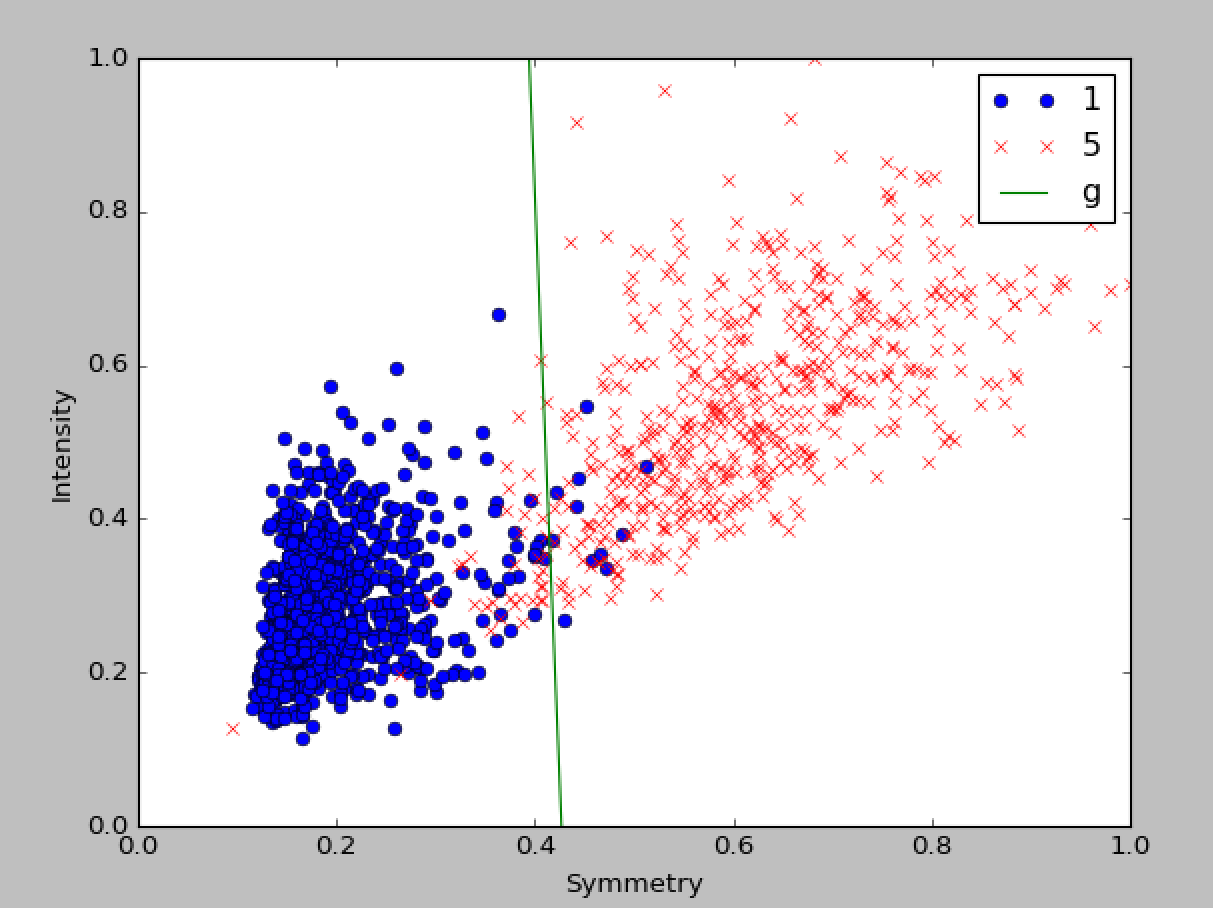
\includegraphics[scale=.75]{1a1.png}
	\\ This is the graph for the training data. The final outputted hypothesis was $g = -30.565x + 13.05$.
	\\ \\ 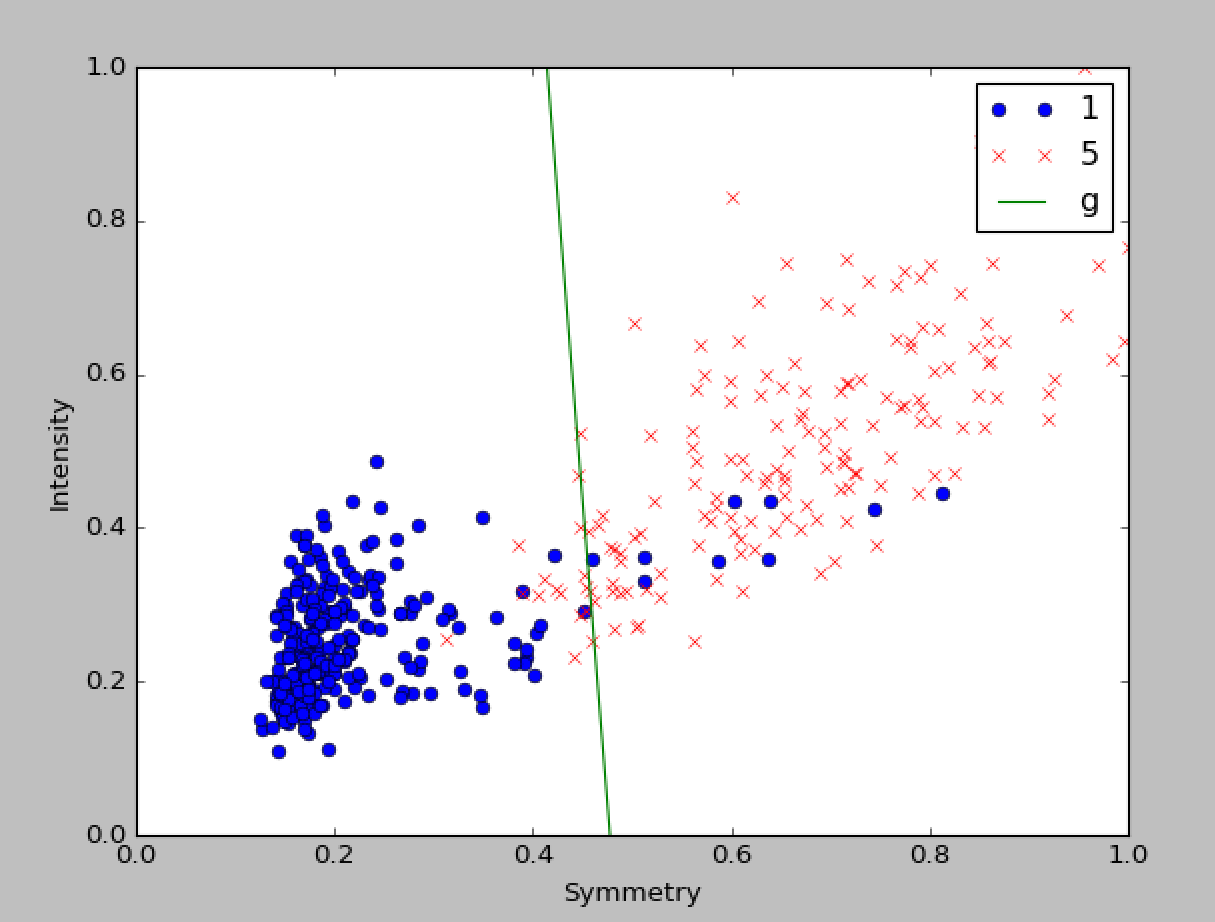
\includegraphics[scale=.75]{1a2.png}
	\\ This is the graph for the test data. The final outputted hypothesis was $g = -15.75x + 7.52$.
	\item $E_{in} = \boldsymbol{0.0805}$ and $E_{test} = \boldsymbol{0.111}$. This was calculated by using a simple squared error summation, where $y_{train} = +1$ for ones and $y_{train} = -1$ for fives.
	\item From class we know that the $d_{VC}$ for a linear hypothesis is $d + 1$. Since this is a 2-d model, $d_{VC} = 3$. We can then apply the error bound that we calculated earlier in Chapter 2 with $\delta = 0.05$, $N = 484$, and $d_{VC} = 3$:
	\begin{gather*}
		E_{out}(g) \le E_{in}(g) + \sqrt{\frac{8}{N} ln \frac{4((2N)^{d_{VC}} + 1)}{\delta}}
		\\ E_{out}(g) \le E_{in}(g) + .64292
		\\ E_{out}(g) \le \boldsymbol{.7234}
 	\end{gather*}
 	However, if we're only testing a single hypothesis on a completely random set of data points (the new test set), we can simply use Hoeffding bound for the error bar from the test set, with $\epsilon = \delta = .05$.
 	\begin{gather*}
	 	P[|E_{out} - E_{in}| > \delta] \le 2e^{-2\delta^2N}
	 	\\ \implies E_{out} \le E_{test} + 2e^{-2\delta^2N}
	 	\\ E_{out} \le E_{test} + .177
	 	\\ E_{out} \le \boldsymbol{.288}
 	\end{gather*}
 	The test error bar is the better bar by far. This makes sense, because here we're dealing with a single hypothesis rather than the set of all linear hypotheses.
 	\item The following graphs were created by replacing each vector $[1, x_1, x_2]$, where $x_1$ is the symmetry of point $x$ and $x_2$ is the intensity of point $x$, with $[1, x_1, x_2, x_1^2, x_1x_2, x_2^2, x_1^3, x_1^2x_2, x_2^2x_1, x_2^3]$. The linear gradient descent algorithm was then run, with 100000 iterations, on this new 10-dimensional space.
 	\\ 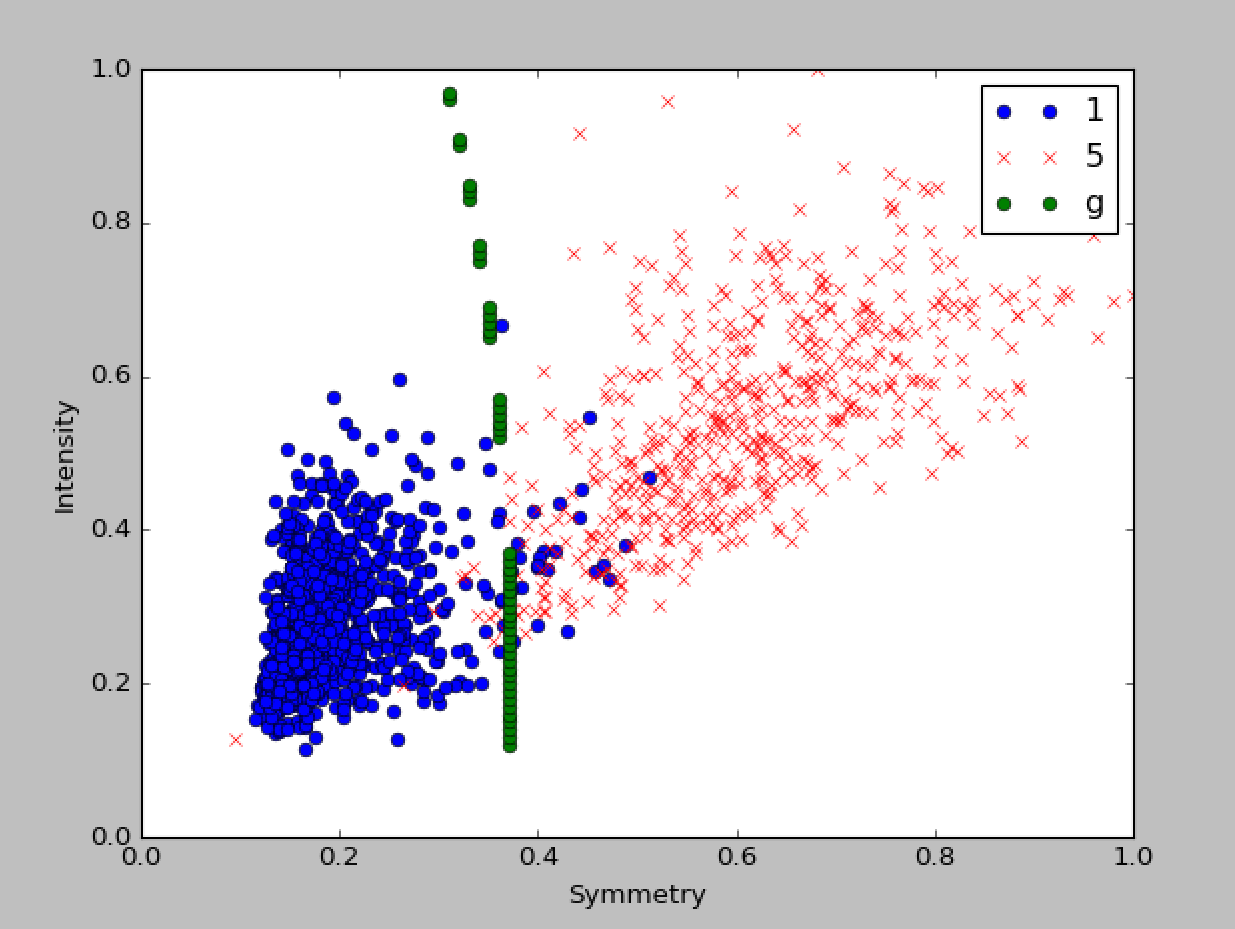
\includegraphics[scale=.5]{1-4b.png}
 	\\ The above graph is what happens when the algorithm is run on the training data. The outputted final hypothesis, g: $0 = 1.65 - 3.79x_1 + x_2 - 4x_1^2 - 3.04x_1x_2 - 0.83x_2^2 + 5.06x_1^3 + 2.73x_1^2x_2 + 1.07x_2^2x_1 - 0.08x_2^3$, with $E_{in} = \boldsymbol{0.0566}$. (The only way I could really think to graph this was by finding points where the above equation is close to 0 iteratively. You can pretty much fill in the gaps for the rest of the hypothesis).
 	\\ 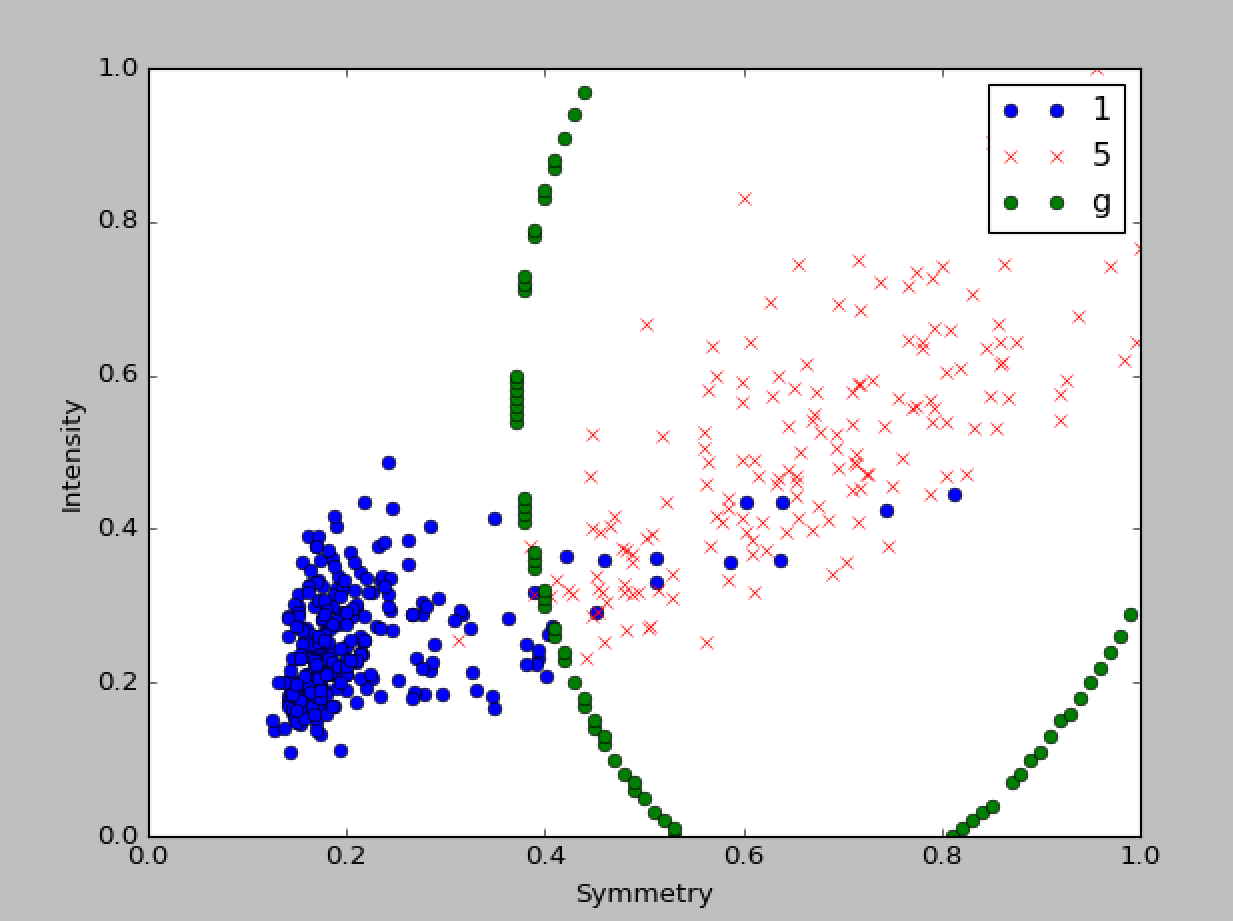
\includegraphics[scale=.5]{1-4a.png}
 	\\ The above graph is from the output on the test set. The outputted final hypothesis, g: $0 = 1.8 - 3.5x_1 + .14x_2 - 2.19x_1^2 - 3.6x_1x_2 - 0.11x_2^2 + 4.71x_1^3 + 0.86x_1^2x_2 + .04x_2^2x_1 + 1.21x_2^3$, with $E_{in} = \boldsymbol{0.0874}$.
 	\\ 
 	\\ \\ We can calculate the error bars based off of these new hypotheses in the same way we did without the transform (accounting for the new $d_{VC}$, of course):
 	\begin{gather*}
 			E_{out}(g) \le E_{in}(g) + \sqrt{\frac{8}{N} ln \frac{4((2N)^{d_{VC}} + 1)}{\delta}}
 			\\ E_{out}(g) \le E_{in}(g) + 1.14999
 			\\ E_{out}(g) \le \boldsymbol{1.21}
 	\end{gather*}
 	This is a terrible error bar, but at least we can look forward to the test bar:
 	\begin{gather*}
	 	P[|E_{out} - E_{in}| > \delta] \le 2e^{-2\delta^2N}
	 	\\ \implies E_{out} \le E_{test} + 2e^{-2\delta^2N}
	 	\\ E_{out} \le E_{test} + .177
	 	\\ E_{out} \le \boldsymbol{.265}
 	\end{gather*}
 	\item I would most likely deliver the \textbf{first order model}. It's instructive to give the above error bars as an exercise, but in reality we cannot truly use Hoeffding bounds on the test set just because we've data snooped a lot. The fact that I can look at the error bar for the linear model test set and for the 3rd order polynomial test set and pick the latter means that my hypothesis set was of size two, not of size one.
 	\\ \\ Additionally, even with a slightly better $E_{in}$, we start running into the risk of possibly overfitting the data because this data is pretty well separable with the simplest model (the Occam's Razor argument).
\end{enumerate}

\section*{Problem 2}
\begin{enumerate}[label=(\alph*)]
	\item First, the gradient descent function was set to have step size 0.01 and run for 50 iterations starting from $(0.1, 0.1)$. The following plot of iterations vs. $f(x)$ was created:
	\\ 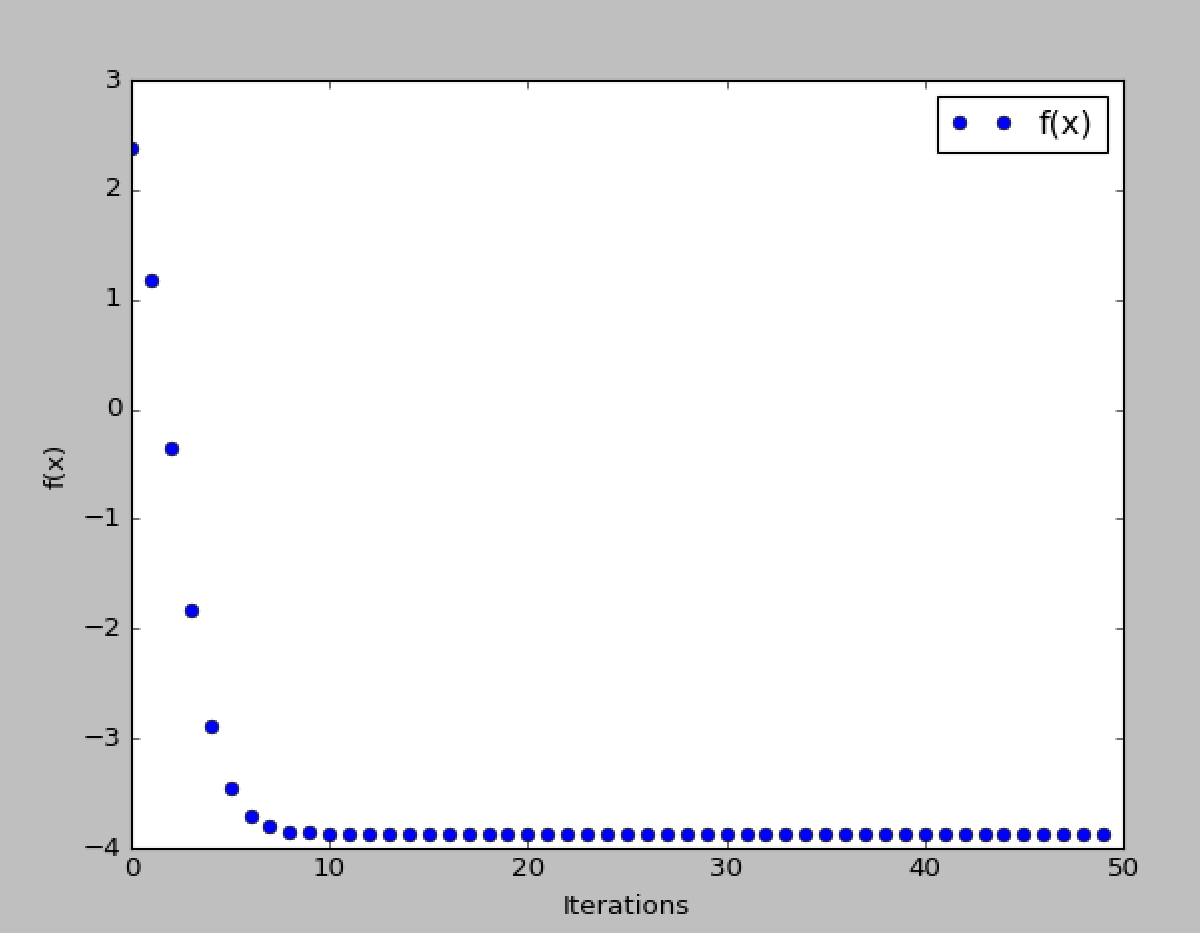
\includegraphics[scale=.5]{2a1.png}
	\\ The final algorithm outputted the point: $\boldsymbol{(-0.238, -0.238)}$ with a final $f(x)$ of $\boldsymbol{-3.88}$
	\\ \\ Then, the step size was changed to 0.1 and rerun with the same number of iterations and starting point, creating the following plot:
	\\ 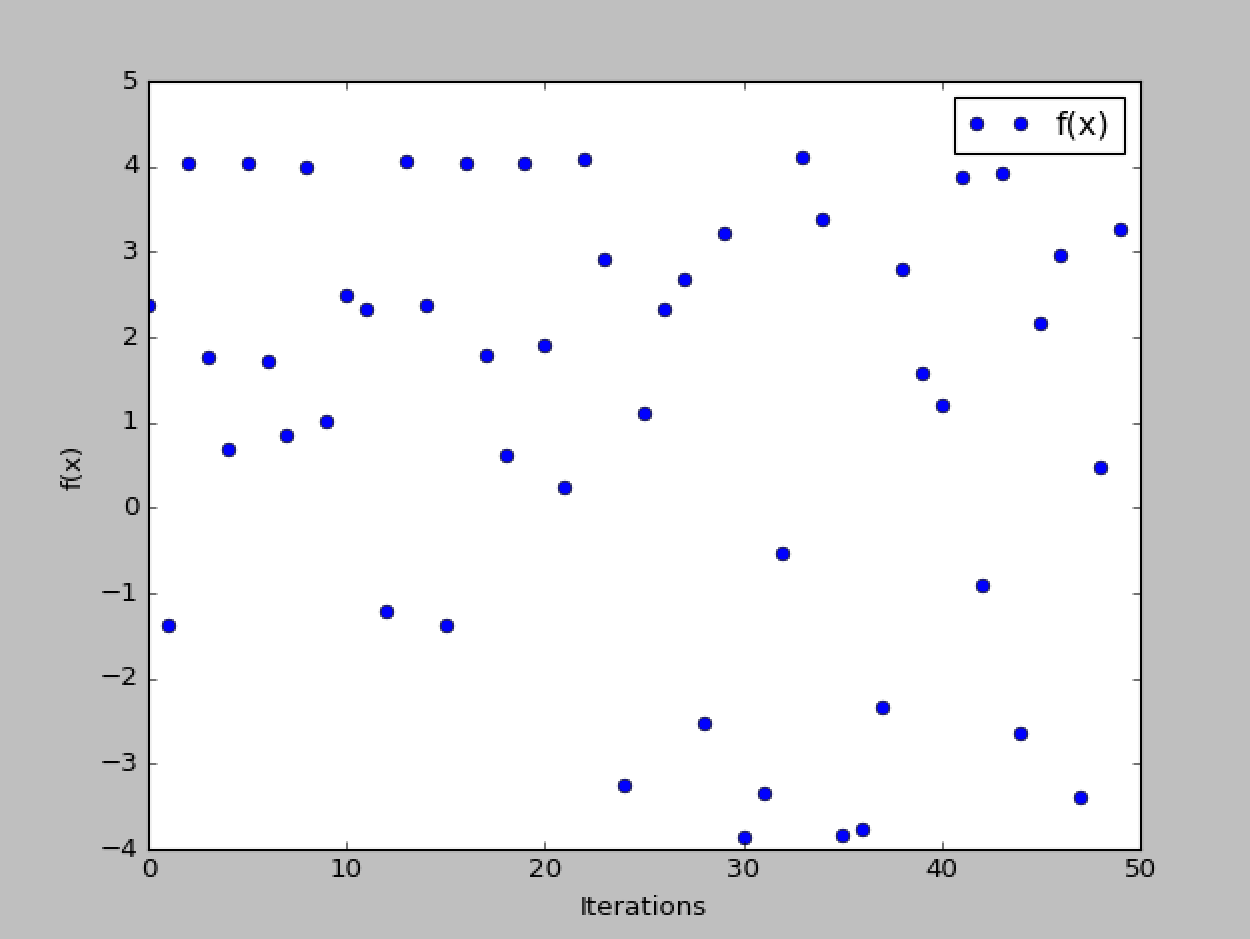
\includegraphics[scale=.5]{2a2.png}
	\\ The final algorithm outputted the point: $\boldsymbol{(-0.0011, -0.0011)}$ with a final $f(x)$ of $\boldsymbol{3.28}$. This is clearly wildly wrong, especially considering it is pretty easy to come up with any number lower ($f(0, 0) = 0^2 + 0^2 + 2 sin(0) + 2 sin(0) = 0$, for instance). This happens because the step size is too large. The gradient descent algorithm sees a local gradient then overreacts by jumping all the way over to another part of the plot.
	\item The gradient descent algorithm was then run on a variety of starting points with both step sizes (0.1, 0.01), and the final f(x)s are listed below in the table. Each time, the algorithm was run for 50 iterations.
	\begin{center}
		\begin{tabular}{| l | l | l |}
			\hline
			\textbf{Starting Pt} & $\eta = \boldsymbol{0.01}$ & $\eta = \boldsymbol{0.1}$ \\ \hline
			$(0.1, 0.1)$ & $-3.88$ & $3.28$ \\ \hline
			$(1, 1)$ & $-2.88$ & $-0.5$ \\ \hline
			$(-0.5, -0.5)$ & $-3.88$ & $-3.43$ \\ \hline
			$(-1, -1)$ & $-0.88$ & $3.88$ \\
			\hline
		\end{tabular}
	\end{center}
	Clearly this is all over the place, and the only reason we know that $-3.88$ is probably the lowest is because we were lucky earlier in choosing starting points.
\end{enumerate}

\section*{Problem 3.16}
\begin{enumerate}[label=(\alph*)]
	\item The expected cost of something happening is equal to its cost multiplied by the probability of it happening. Fortunately, we are given both of those as logistic regression outputs probabilities from 0 to 1.
	\\ \\ We only incur an accept cost if the algorithm was wrong on a specific data point $x$. The probability of this happening is $1 - g(x)$, because we computed $g(x)$ to be the probability of the person being correct. As a result, $cost(accept) = [1 - g(x)]c_a$.
	\\ \\ Similarly, we only incur a reject cost if the algorithm was wrong on a specific data point. The probability of this happening is $g(x)$, because we computed $1 - g(x)$ to be the probability of the person being an intruder. As a result, $cost(reject) = g(x)c_r$.
	\item We should put the threshold at the $g(x)$ value where the costs are equal. This is because if, for any of the data points, either of the costs is larger, we should clearly go with that option.
	\begin{gather*}
		cost(reject) = cost(accept)
		\\ (1 - g(x)) c_a = g(x) c_r
		\\ c_a - g(x) c_a = g(x) c_r
		\\ g(x) (c_r + c_a) = c_a
		\\ g(x) = \frac{c_a}{c_r + c_a}
	\end{gather*}
	\item For the Supermarket, $c_a = 1$ and $c_r = 10 \implies \kappa = \frac{c_a}{c_a + c_r} = \frac{1}{1 + 10} = \boldsymbol{\frac{1}{11}}$
	\\ \\ For the CIA, $c_a = 1000$ and $c_r = 1 \implies \kappa = \frac{c_a}{c_a + c_r} = \frac{1000}{1000 + 1} = \boldsymbol{\frac{1000}{1001}}$
\end{enumerate}
\end{document}